\chapter{Trabalho relacionado} \label{cap:trabrelacionado}
Este cap�tulo apresenta uma vis�o do estado da arte relacionado com a seguran�a 
e modelos de simula��o em RSSF. A primeira sec��o apresenta a caracteriza��o de
uma RSSF, permitindo real�ar as limita��es destas redes nomeadamente no que diz
respeito ao modelo de energia. A segunda sec��o apresenta a defini��o do modelo
de advers�rio e tipologias de ataques. A terceira sec��o apresenta protocolos de
encaminhamento seguro. A ultima sec��o apresenta diversos ambientes de simula��o
relacionados com as RSSF e \textit{ad-hoc}. 
\section{Caracteriza��o de uma RSSF}\label{sect:subsec_arq_sofware_wsn}
Nas RSSF podem-se considerar v�rios tipos de n�s de computa��o, estando estes 
interligados por uma infraestrutura de comunica��o textit{multi-hop}, em que
cada n� da rede (\textit{mote}) pode desempenhar pelo
menos tr�s papeis\cite{REFERENCIA} : 1) N� gerador de dados, pela capta��o da
eventos associados �s especificidades dos sensores possu�dos; 2) N�
encaminhador, que recebendo dados de uns n�s os encaminha  para outros por forma
a que alcancem o destino; 3) N� de sincroniza��o ou n� de agrega��o, embora
estas duas caracteriza��es n�o correspondam � mesma tarefa, por si s�, a um
n�vel mais macro, corresponde igualmente a colec��o de dados da rede e a um
pr�-processamento, por forma a faz�-los seguir de forma agregada para outro
destino (interno ou externo � rede ).
\subsection{Modelo da plataforma gen�rica de uma RSSF - \textit{Mote}} 
Interessa perceber qual a arquitectura inerente a estas plataformas de rede, 
onde � poss�vel executar uma multiplicidade de aplica��es, apesar das limita��es
impostas pela arquitectura. Na figura seguinte apresenta-se um modelo
simplificado\cite{ livro_wsn_arch} que ilustra os diversos componentes que
concorrem para o funcionamento de um \textit{mote} numa RSSF. 
\begin{center}
\begin{figure}[ht]
\centering
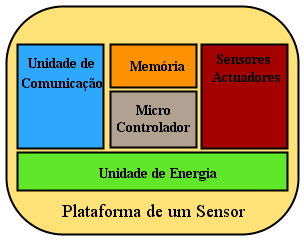
\includegraphics[height=5cm,width=7cm]{SENSOR_NODE.png}
\caption{Modelo de um Sensor de uma RSSF (baseado em
\cite{LIVROARCH_WSN})} \label{fig:sensor_mode}

\end{figure}
\end{center}
Como se pode observar na \figurename \ref{fig:sensor_node}, os sistemas que 
est�o presentes s�o os seguintes:  i) Sistema de processamento;  ii) Sistema de
comunica��o; iii) Sistema sensorial; iv) Sistema de mem�ria; v) Sistema de
energia;. 
\paragraph{Sistemas de processamento}
O sistema de processamento � um componente essencial num 
\textit{mote}\cite{Holger_Karl_protocols_andarchs_wsn}. Toda o conjunto de
processamento pode ser realizado nas v�rias arquitecturas representando um
\textit{trade-off} entre desempenho, flexibilidade, performance, custo e consumo
de energia. Dois dos processadores mais utilizados nas redes de
sensores actuais s�o os da tecnologia Atmel Atmega 128L \cite{atmel} e da Texas
Instruments o controlador TI MSP430 \cite{TIMSP430}

\paragraph{Sistemas de comunica��o}
Este sistema � o respons�vel pela transfer�ncia de dados entre diversos n�s de 
uma rede por interm�dio de radio frequ�ncia, o que quer dizer sem fios. A
r�dio-frequ�ncia permite ter bom alcance de comunica��o com boas taxas de
transfer�ncia, bem como equilibrar o consumo de energia perante exist�ncia de
erros. 

Os transmissores e receptores \footnote{No caso da implementa��o em
RSSF, as plataformas incorporam num mesmo componente as duas fun��es,
transmiss�o e recep��o, estes s�o denominados por \textit{transceivers}}nos n�s 
t�m a fun��o de transformar uma cadeia de bits, vindas do processador, em
ondas electromagn�ticas. Os estados pelos quais passam estes componentes s�o os
seguintes e est�o associados essencialmente ao consumo de energia: a
trasmitir\footnote{o transmissor est� activo e a emitir
dados}, a receber\footnote{O receptor est� activo e a receber dados},
\textit{idle}\footnote{Est� livre para  receber dados, note-se que alguns
componentes de comunica��o est�o activos e outros est�o desligados},
\textit{sleep}\footnote{A maior parte dos componentes de comunica��o est�o
desligados}.  Alguns dos sistemas de r�dio existentes nas redes de sensores s�o
os seguintes: Xemics XE1205 \cite{XEMICS XE1205}, Chipcon 2420 (com chipset para
802.15.4)\cite{CHIPCON2420}.

Porque o custo energ�tico da comunica��o tem uma ordem de grandeza bastante 
superior ao do processamento, o existe uma liga��o estreita entre o sistema de
comunica��o e o protocolo de acesso ao meio (MAC)\cite{mac_protocols}. Estes
protocolos, permitem optimizar o tempo de opera��o do sistema de comunica��o,
com vista � redu��o do consumo de energia permitindo aumentar o tempo de vida
�til de uma RSSF. 

\paragraph{Sistemas Operativos} 
Os sistemas operativos (SO's) para as RSSF s�o menos complexos do que os 
restantes SO's comuns para PC's. De seguida apresentam-se alguns
sistemas operativos com vista a contribuir para a compreens�o do estado da arte
nesta componente das RSSF.
\begin{description}
 \item[TinyOS\cite{tinyos}] Sistema operativo livre e de c�digo aberto, 
desenvolvido pela Universidade da California, Berkeley e implementado em nesC
(uma extens�o da linguagem C) muito optimizado para as limita��es de mem�ria
existentes nas RSSF. O modelo de execu��o orientado por eventos possibilita uma
maior precis�o na gest�o de energia, ainda assim tem grande flexibilidade no
escalonamento dos eventos gerados pelo ambiente real, que, como se sabe, s�o de
natureza muito imprevista.
 \item[Contiki\cite{Contiki}] Sistema operativo livre e de c�digo aberto, 
implementado em C, e tal como o TinyOS\cite{TinyOS} � orientado por eventos. As
aplica��es podem ser carregadas e descarregadas em tempo de execu��o. Os
processos deste SO usam \textit{threads} leves, denominadas por protothreads
que proporciona um estilo de programa��o  \textit{threadlike} em cima do
\textit{kernel} orientado a eventos.
 \item[Nano-RK\cite{nanork}] Sistema operativo desenvolvido na universidade  de
Carnegie Mellon, o seu \textit{kernel} � baseado em execu��o em tempo real com 
\textit{multithreading } preemptivo. Assim � possivel ao \textit{kernel} 
controlar que processos t�m acesso ao CPU, com a divis�o em frac��es de tempo a
que cada processo acede ao CPU, � rede e aos sensores.
 \end{description}
 \paragraph{Sistemas de energia}
A energia � um recurso escasso e como tal deve ser tido em conta no desenho  de
uma qualquer RSSF, adaptando-se � aplica��o ou aos eventos que se pretendem
monitorizar. Assim, os dispositivos fornecedores de energia podem ser de
diversos tipos, por exemplo: baterias (tipo AA), baterias fotovolta�cas .
Encontra-se nas especifica��es das plataformas mais recentes os valores que
indicam o consumo energ�tico nos diversos estados de opera��o de um
\textit{mote} a titulo de exemplo observe-se a plataforma
\textit{Mica2}\cite{MICA} da \textit{Crossbows}\cite{CrossbowSite}:


\begin{table*}[ht]
\centering % used for centering table
\begin{tabular}{l r} % centered columns (4 columns)
\hline\hline %inserts double horizontal lines
Descri��o & Valor \\ [0.5ex] % inserts table
%heading
\hline % inserts single horizontal line
Baterias& 2xAA \\ % inserting body of the table
M�nimo $V_{in}$ & 2.7 V \\
Capacidade da bateria& 2000 mAh \\
Regulada &  no \\
\hline %inserts single line
\end{tabular}
\label{table:mica2_caracter} % is used to refer this table in the text
 \caption{Caracter�sticas de energia do \textit{mote} Mica2
(origem:\cite{mica2_datasheet}))} % title of Table
\end{table*}

\begin{table*}[ht]
\centering % used for centering table
\begin{tabular}{l r} % centered columns (4 columns)
\hline\hline %inserts double horizontal lines
Opera��o & Consumo\\ [0.5ex] % inserts table
%heading
\hline % inserts single horizontal line
CPU \textit{sleep} com \textit{timer} \textit{on} & 0.054 mW \\ % inserting body
CPU activo,\textit{ radio }\textit{off} & 36 mW \\
CPU activo, \textit{radio idle listening }& 66 mW \\
CPU activo, \textit{radio TX/RX }& 117 mW \\
Pot�ncia M�xima (CPU activo, radio TX/RX + flash write) & 165 mW \\ [1ex] %
%[1ex] adds \hline %inserts single line
\end{tabular}
\label{table:mica2_powerops} % is used to refer this table in the text
 \caption{Consumo de Energia \textit{Mica2} - Opera��o Tipica
(origem:\cite{mica2_datasheet})} % title of Table
\end{table*}


\subsection[]{Modelo de energia de uma RSSF} 
Nas diversas aplica��es das RSSF\cite{APPLICA��ES}, uma das caracter�sticas que
tornam estas redes como as mais aconselhaveis para o seu uso � a capacidade de
auto-organiza��o, de facilidade de distribui��o por locais remotos e de grande
dimens�o, permitindo a monitoriza��o de eventos durante o maior tempo poss�vel.
Assim, para al�m das preocupa��es referentes � seguran�a e correc��o de recolha
dos dados, a energia � uma problem�tica relevante e que deve ser considerada em
todos os momentos. Desde logo os sensores j� possuem, na sua arquitectura,
servi�os que visam a optimiza��o da energia, permitindo que o tempo de vida �til
da rede seja estendido o mais poss�vel. Durante o seu funcionamento, um qualquer
n� sensor, passa cerca de 90\% do tempo num estado "adormecido", o que implica a
inactiva��o de alguns dos seus componentes com vista a redu��o do consumo de
energia\cite{energia}. Note-se que este comportamento � poss�vel devido �
natureza das pr�prias aplica��es das RSSF, por exemplo, se o n�mero de eventos
detectados e propagados pela rede tiver uma frequ�ncia de acontecimento muito
grande, naturalmente o tempo neste estado de adormecimento ter� tend�ncia a ser
reduzido. No entanto o comportamento esperado numa RSSF � a ocorr�ncia espa�ada
de eventos, permitindo por isso que um n� passe a maior parte do tempo num
estado em que o consumo de energia seja m�nimo. 

Existem v�rios protocolos de acesso ao meio (MAC) que implementam estas mudan�as
de estado que podem ser completamente aut�nomas, ou seja n�o exigindo a
coordena��o com os n�s vizinhos, ou de forma coordenada em que a informa��o
trocada com os vizinhos contribui para passar mais ou menos tempo em estados de
adormecimento\cite{MACs}.
Considera-se que existem tr�s estados principais na opera��o de um sensor:
activo, inactivo, adormecido.  No primeiro estado, poder-se-�o considerar,
ainda,  diferentes modos de funcionamento, devido aos componentes de um n�
sensor estarem ligados ou desligados em determinado momento e com isso 
consumirem mais ou menos energia. Na tabela seguinte apresenta-se alguns dos
estados considerados numa plataforma do tipo Mica2\cite{mica2}.

FALTA TABELA AQUI

A energia nas RSSF � tida em considera��o desde a implementa��o do \textit
{hardware} at� ao desenho e implementa��o de qualquer dos servi�os existente na
pilha de software dos n�s sensores. T�m se observado que a maioria dos estudos
desenvolvidos s�o levados a cabo com recurso a ambientes de
simula��o\cite{Germano_Guimar�es,outros} estes ambientes ou ferramentas que
permitem o estudo dos perfis de consumo de energia numa RSSF, s�o calibrados com
recurso �s especifica��es dos fabricantes \cite{} e a resultados de experi�ncias
em sensores reais. O estudo desta problem�tica � ainda mais relevante quando se
associa a problem�tica da seguran�a na opera��o das RSSF.
Dos componentes de um \textit{mote}, o sistema de comunica��o e o CPU s�o os que
mais influenciam o consumo de energia. Ainda o maior peso seja dado para a
comunica��o, numa ordem de grandeza de 1 para 1000  face ao processamento.
Quando se pretendem introduzir mecanismos de seguran�a ao n�vel do
encaminhamento de dados, � necess�rio ter presente que existe um custo a pagar
no que respeita � energia, devendo-se este facto ao aumento da computa��o, uma
vez que est�o envolvidas opera��es de criptografia\cite{PAPERS_CRIPTENERGIA} e
mesmo ao n�vel da comunica��o caso os modos de criptografia aumentem o tamanho
das mensagens enviadas\cite{PAPERS_ENERGIA}. Conhecidas as limita��es impostas
pela arquitectura, algumas derivadas da pequena dimens�o dos sensores,
poder-se-� dizer que os protocolos de acesso ao meio representam um papel
importante no consumo de energia\cite{MAC_ENERGIA}. 
\section{Modelo de Advers�rio, Ataques ao Encaminhamento e
Contra-medidas} \label{sect:sec_mod_adversario_ataq_contramedidas}
\subsection{Arquitectura de Servi�os de Seguran�a em RSSF} \label{sect:subsec_arq_security_wsn}
Num sistema seguro � necess�rio que a seguran�a esteja integrada em cada um dos seus componentes, 
n�o se confinando a um componente isolado do sistema \cite{sec_in_wsn_perrig}. Nesta sec��o,
apresenta-se, introdutoriamente, alguns requisitos de seguran�a de uma RSSF e 
alguns servi�os de seguran�a, que representam um ponto de
partida para a garantia de propriedades de seguran�a, aquando do desenho de RSSF seguras.
\subsubsection{Requisitos de seguran�a de uma RSSF}
Os requisitos de seguran�a de uma RSSF podem variar consoante as especificidades da aplica��o que a
rede visa suportar. No entanto, apresentam-se, de forma gen�rica, os principais requisitos de
seguran�a de uma RSSF \cite{sec_in_wsn_perrig}:
\begin{descriptionNoIndent}
\item[Autentica��o]
Sendo que o meio de comunica��o � partilhado, � necess�rio recorrer � autentica��o para garantir a
detec��o de mensagens alteradas ou injectadas no sistema, de forma n�o autorizada
\cite{sec_in_wsn_perrig}. O uso de criptografia assim�trica ainda n�o � vi�vel nas RSSF,
considerando as limita��es destas redes e as exig�ncias computacionais\footnote{N�o somente em
termos de mem�ria, mas tamb�m em termos de energia} destes mecanismos;
 \item[Confidencialidade]
Sendo uma RSSF uma infraestrutura baseada, fundamentalmente, na dissemina��o de dados recolhidos
sensorialmente em ambiente remoto e/ou n�o controlado e, normalmente, de f�cil acesso, � necess�rio
garantir a confidencialidade dos dados que circulam na rede. O uso de criptografia � o mais
indicado para este tipo de protec��o, sendo adequada a selec��o de algoritmos de encripta��o
fi�veis (ex: AES\footnote{\textit{Advanced Encryption System}} \cite{Stallings2005},
ECC\footnote{\textit{Elliptic Curve Cryptography}}\cite{Stallings2005}. Com a utiliza��o de chaves
criptogr�ficas, � necess�ria a adop��o de esquemas seguros de distribui��o de chaves
\cite{eschenauer2002}.
 \item[Disponibilidade]
Entende-se por disponibilidade a garantia do funcionamento de uma rede durante a totalidade do tempo
de opera��o. Os ataques que visam afectar esta propriedade s�o denominados por ataques de nega��o de servi�o (\textit{Denial of Service} - \textit{DoS}) \cite{Hu2005}. 
Para al�m de mecanismos que evitem estes ataques, � necess�rio garantir que a degrada��o da rede (na presen�a de um ataque ) � controlada, ou seja, � proporcional ao n�mero de n�s
comprometidos; 
 \item[Integridade]
A integridade garante que os dados recebidos por um n� n�o s�o alterados, por um
atacante, durante a transmiss�o. Em alguns casos, esta propriedade � garantida juntamente com a
autentica��o, usando mecanismos que permitem garantir ambas as propriedades numa s� opera��o. � comum o
uso de CMAC \footnote{\textit{Cipher based Message Authentication Code}} \cite{Stallings2005}, uma
vez que permite autenticar (com o uso de chave criptogr�fica sim�trica) e verificar a
integridade de uma mensagem \cite{SPINS}.
\item[Detec��o de Retransmiss�o Il�cita (ou Teste de Frescura da Mensagem)]
A frescura de uma mensagem garante que n�o � antiga
e/ou n�o foi reenviada por um atacante \cite{SPINS,Luk2007d}. Podem-se considerar dois
tipos de frescura: fraca (garantindo ordem parcial e sem informa��o do desvio de tempo,
usada para as medi��es dos sensores) e forte (que garante ordem total em cada
comunica��o, permitindo estimar o atraso, sendo usada para a sincroniza��o de tempo).
 \end{descriptionNoIndent}
\subsubsection{Servi�os B�sicos de Seguran�a}\label{sec:servicos_basicos_de_seguranca}
Alguns servi�os de seguran�a t�m vindo a ser desenvolvidos para as RSSF, com vista a garantir a
seguran�a ao n�vel da comunica��o (ex: criptografia, assinaturas, \textit{digests}). Estes servi�os
permitem que o arquitecto de sistemas se centre noutras problem�ticas relacionadas com o
comportamento dos protocolos face a ataques, por exemplo, de intrus�o. Apresentam-se de seguida
alguns servi�os mais comuns que representam as arquitecturas b�sicas de seguran�a para RSSF:
\begin{descriptionNoIndent}
\item[TinySec \cite{Karlof2004}]
TinySec � uma arquitectura para protec��o ao n�vel de liga��o de dados em RSSF. O objectivo
principal � o de providenciar um n�vel adequado de seguran�a, com o m�nimo consumo de recursos. Os
servi�os de seguran�a  disponibilizados s�o: autentica��o de dados (com a utiliza��o de
\textit{Message Authentication Codes}(MAC) \cite{Stallings2005}, em
particular o CBC-MAC\footnote{Cipher Block Chaining - Message Authentication Code (CBC-MAC))}) e
confidencialidade (CBC-MAC). N�o implementa nenhum mecanismo que garanta a frescura das mensagens,
tornando-o vulner�vel a ataques de retransmiss�o il�cita;
\item[MiniSec \cite{Luk2007d}]
Minisec � uma camada de rede concebida para possuir baixo consumo de energia (melhor que o
TinySec) e alta seguran�a. Uma das caracter�sticas principais, que a tornam mais eficiente, � o uso
do modo \textit{Offset Codebook} (OCB) \cite{Stallings2005} para encripta��o de blocos. Desta forma, � poss�vel, numa �nica passagem, autenticar e encriptar os dados, sem aumentar o tamanho da
mensagem, contribuindo para um menor consumo de energia. Esta arquitectura tem dois modos
de opera��o: um orientado para comunica��o \textit{unicast} (MINISEC-U) e outro para comunica��o 
\textit{broadcast} (MINISEC-B);
\item[SPINS \cite{SPINS}]
Conjunto de protocolos de seguran�a, constitu�do por dois componentes
principais: SNEP\footnote{Secure Network Encryption Protocol} \cite{SPINS} e
${\mu}$TESLA  \cite{SPINS,Luk2006}. O primeiro fornece servi�os de autentica��o e
confidencialidade \textit{unicast}, encriptando as mensagens (com
o modo CTR\footnote{\textit{Counter Mode}}) e protegendo-as com um MAC (CBC-MAC). O
SNEP gera diferentes chaves de encripta��o que derivam de uma chave-mestra, partilhada entre 
dois n�s, com um contador de mensagens para garantir a frescura de cada mensagem. O segundo componente, o
${\mu}$TESLA \cite{SPINS,Luk2006}, � um servi�o de autentica��o de \textit{broadcast}, que evita a
utiliza��o de mecanismos mais exigentes, de criptografia assim�trica, recorrendo a criptografia
sim�trica, autenticando as mensagens com um CMAC;
\item[Norma IEEE802.15.4 \cite{ietf_802154}]
Esta norma define a especifica��o da camada f�sica e de controlo de acesso ao meio das redes
pessoais de baixa pot�ncia (\textit{LRPAN}\footnote{Low Rate Personal Area Networks}). Foca-se,
essencialmente, na comunica��o entre dispositivos relativamente pr�ximos, sem a
necessidade de uma infraestrutura de suporte, explorando o m�nimo de consumo de energia. � uma norma
que j� se encontra implementada em algumas plataformas das RSSF (ex: Micaz \cite{micaz}).
Especifica alguns servi�os de seguran�a \cite{zigbee_802154},  representando uma primeira
linha de protec��o contra ataques � infraestrutura. Estes mecanismos s�o os seguintes: i) Cada
dispositivo mant�m uma lista de controlo de acessos (ACL) dos dispositivos confi�veis,
filtrando comunica��es n�o autorizadas; ii) Encripta��o de dados, partilha de uma chave
criptogr�fica entre os intervenientes na comunica��o; iii) Servi�o de integridade de cada
\textit{frame}, adicionando a cada \textit{frame} um \textit{Message Integrity Code}
(MIC) \cite{Stallings2005}; iv) Garantia de frescura de mensagens (\textit{Sequential Freshness}),
utilizando contadores de \textit{frames} e de chaves.
\item[ZigBee \cite{zigbee_802154,zigbee}]
Com a norma 802.15.4, orientada para as duas camadas mais baixas da pilha de
protocolos das RSSF, a norma ZigBee define as especifica��es para
a camada de rede e de aplica��o. J� incorpora alguns servi�os de seguran�a, nomeadamente: i)
Frescura, mantendo contadores associados a cada chave de sess�o, que s�o reiniciados em cada mudan�a
de chave; ii) Integridade, com op��es de integridade de mensagens que v�o desde os 0 aos 128 bits de
verifica��o; iii) Autentica��o, ao n�vel de rede e ao n�vel de liga��o de dados; iv)
Confidencialidade, com o algoritmo AES \cite{Stallings2005} com 128 bits.
Esta arquitectura utiliza o conceito de \textit{trusted center} para gest�o da seguran�a na rede,
implementando um coordenador de rede ZigBee. Este, acreditado por todos os n�s da rede, pode
desempenhar tr�s fun��es: i) Autentica��o de n�s participantes na rede; ii) Manuten��o e
distribui��o de chaves; iii) Seguran�a ponto-a-ponto entre n�s da rede.
\end{descriptionNoIndent}

\subsection{Modelo de Advers�rio} \label{sect:sec_mod_adversario_serv_seg}
A defini��o do modelo de advers�rio permite, desde logo, identificar as caracter�sticas e as 
capacidades dos atacantes e os ataques que estes podem desencadear na rede. Nesta sec��o,
caracteriza-se o modelo de advers�rio que enforma este trabalho.
\subsubsection{Modelo de Dolev-Yao}\label{sect:subsec_dolev_yao}
Um dos modelos de advers�rio mais conhecidos, quando se trata de an�lise formal de protocolos
seguros, � o modelo de Dolev-Yao \cite{Dolev1983}. Neste modelo, � considerado que a rede est�
sobre
o dom�nio do advers�rio o qual, perante este facto, pode extrair, reordenar, reenviar, alterar e
apagar
as mensagens que circulam entre quaisquer dois n�s leg�timos. Com esta assump��o, entende-se
portanto, que o advers�rio transporta a mensagem e, com isso, adopta um ataque do tipo 
\textit{man-in-the-middle} \cite{Stallings2005}, com comportamento incorrecto. Este funcionamento,
entenda-se, n�o � comparado � intrus�o mas sim � intercep��o de mensagens e pode ser mitigado pela
utiliza��o de mecanismos de criptografia.

As tipologias de ataque consideradas pelo modelo de advers�rio de Dolev-Yao
s�o  instanciadas pela norma X800 \cite{ITU-T1991}, que pretende
normalizar
uma arquitectura de seguran�a para o modelo OSI \cite{sd_tanenbaum}, atrav�s de uma abordagem
sistem�tica para o desenho de sistemas seguros. Esta norma considera a seguran�a
sob tr�s aspectos: ataque, mecanismo e servi�o de
seguran�a \cite{Stallings2005}. O
primeiro refere-se � forma usada para comprometer um sistema, por exemplo,
alterando ou tendo acesso n�o autorizado a dados desse sistema\footnote{ Na
literatura, algumas vezes usam-se os termos "ataque" e "amea�a" para denominarem o
mesmo efeito. No entanto, recorrendo ao RFC 2828 \cite{IETF2828}, podemos
definir amea�a como uma potencial viola��o de seguran�a, ou seja, � apenas uma
vulnerabilidade que pode ser explorada para desencadear um ataque. No caso do ataque, trata-se da
explora��o inteligente de uma ou
mais amea�as que resultam na viola��o, com sucesso, de um sistema que se pretendia
seguro}. O segundo aspecto considerado s�o os mecanismos de
seguran�a, que se entendem como o processo que permite detectar, prevenir ou
recuperar de um ataque � seguran�a (ex: encripta��o, controlo de acesso,
assinatura digital) \cite{Stallings2005}. Por fim, o terceiro aspecto define os
servi�os que, fazendo uso de um ou mais mecanismos de seguran�a, permitem resistir a
ataques dirigidos a determinada fonte de informa��o, quer seja durante o
processamento, quer seja durante a comunica��o. Considera-se, ent�o, que, para efeitos da futura
disserta��o,
os ataques subjacentes ao modelo de Dolev-Yao s�o protegidos a partir do estabelecimento de uma
camada b�sica de seguran�a, concretizada por uma das arquitecturas anteriormente referidas na Sec��o
\ref{sec:servicos_basicos_de_seguranca}. 
\subsubsection{Modelo de Intrus�o em RSSF}\label{sect:subsec_intrusao}
Considerando o estudo de seguran�a numa RSSF e, dada a sua exposi��o natural, nomeadamente a f�sica,
colocando cada sensor ao alcance de um advers�rio, torna-se relevante a considera��o de novos
modelos
de advers�rio. Cada rede pode ser constitu�da por milhares de sensores e cada
um destes sensores � um ponto de poss�vel ataque \cite{Perriga}. Este ataque pode ser
tipificado como sendo por intrus�o ou captura. 

Este tipo de ataques pode ser desencadeado desde o n�vel
MAC \cite{Xiao2006} at� ao n�vel de intrus�o f�sica. Neste �ltimo, um actor externo
captura um ou mais sensores leg�timos e descobre os segredos criptogr�ficos. Este
facto permite-lhe replicar \cite{Parno2005} os segredos para sensores maliciosos, 
introduzido-os na rede de modo a que, agindo coordenadamente, possam comprometer a rede.
Conseguida a intrus�o, o atacante pode induzir, nos sensores leg�timos,
comportamentos incorrectos, baseados na informa��o falsa introduzida pelos
sensores maliciosos, influenciando o processo de encaminhamento. Estes ataques s�o de dif�cil
detec��o, uma vez que o car�cter aut�nomo das RSSF pode n�o permitir distinguir um comportamento
errado de uma falha. Com a intrus�o, um
sensor malicioso, embora respeitando o protocolo da rede, pode actuar de forma incorrecta,
levando a rede a criar topologias espec�ficas para determinado ataque ou for�ando toda a
informa��o a passar por n�s maliciosos, podendo estes suprimir ou violar a informa��o. 
\paragraph{Modelo bizantino: advers�rios bizantinos}
O modelo de ataques por intrus�o tem algumas parecen�as com as denominadas falhas
bizantinas \cite{falhas_bizantinas}, que s�o caracterizadas como 
falhas arbitr�rias para com as quais um sistema n�o est�, � partida, preparado para lidar e que se
pode
traduzir em comportamentos inesperados. Transpondo esta realidade para as
RSSF \cite{Fault_Intrusion_Tolerant_Techniques}, � dif�cil
detectar a introdu��o de n�s maliciosos, aut�nomos ou replicados a partir de um n� que foi	
comprometido. No entanto, alguns autores \cite{Parno2005,falhas_bizantinas} t�m-se
debru�ado sobre esta problem�tica, a fim de dotarem os
algoritmos de encaminhamento com mecanismos que permitam detectar a replica��o de n�s maliciosos
numa RSSF.
Para se lidar com ataques com comportamentos bizantinos, recorre-se a mecanismos
probabil�sticos que, ainda que possam n�o mitigar o ataque por completo, aumentam a resili�ncia e
acabam por transformar um ataque num mal menor, definindo at� onde pode ser comprometida a rede, por
forma a garantir a fiabilidade necess�ria para o seu funcionamento.



 

\subsection{Ataques ao Encaminhamento} \label{ataques_encaminhamento}
Apesar de existirem ataques que podem ser dirigidos a qualquer uma das camadas da pilha da RSSF, nesta
sec��o apresentam-se os ataques relacionados com a camada de rede, respons�vel pelo
encaminhamento de dados. Os protocolos de encaminhamento em MANETs \cite{Corson1999} e em RSSF, de
uma forma geral, decomp�e-se em tr�s fases: descoberta dos caminhos, selec��o dos caminhos e
manuten��o da comunica��o pelos caminhos seleccionados. Os ataques a um algoritmo de encaminhamento,
normalmente, podem explorar as vulnerabilidades de cada uma destas fases de forma espec�fica. Em
seguida, os ataques s�o associados � fase do protocolo em que se podem desencadear e s�o
apresentadas, tamb�m, as contra-medidas que permitem mitig�-los.
\subsection{Ataques � organiza��o da rede e descoberta de n�s} \label{sect:subsec_ataq_org_rede}
Nos protocolos do tipo \textit{table-driven} \cite{al-karaki_routing_2004}, ap�s a descoberta dos
n�s vizinhos � necess�rio recolher informa��o para a constru��o das tabelas
de encaminhamento. No entanto, em protocolos do tipo \textit{on-demand}
\cite{al-karaki_routing_2004}, esta fase � desencadeada em cada in�cio de transmiss�o. Este
funcionamento corresponde � organiza��o e descoberta de n�s numa RSSF.
\begin{descriptionNoIndent}
\item[Falsifica��o de Informa��o de Encaminhamento]
Este ataque tem impacte na forma��o da rede e na descoberta dos n�s. Induz a cria��o de entradas
incorrectas nas tabelas de encaminhamento, podendo tamb�m fazer com que estas fiquem lotadas e
inv�lidas. Nos protocolos \textit{on-demand}, o impacte pode ser menor, uma vez que obriga o 
atacante a injectar informa��o errada a cada ciclo de transmiss�o. Outro ataque que causa
estes mesmos efeitos � realizado por n�s atacantes que inundam a rede com pacotes do tipo
\textit{Route Request} (RREQ), pondo em causa a disponibilidade da rede.
\item[Rushing Attacks]
O \textit{Rushing attack} \cite{Rushing_attacks_perrig} � definido pela explora��o, por parte do
atacante, de uma janela de tempo para responder a um pedido de caminho para um destino. Este ataque
� efectivo quando o protocolo (ex:
AODV \cite{Perkins1999}) aceita a primeira resposta que recebe \textit{Route Reply}(RREP).
Explorando isto, o atacante � sempre um candidato a ser o pr�ximo encaminhador, uma vez que n�o
respeita temporizadores nem condi��es de resposta, podendo depois influenciar o estabelecimento das
rotas.
\end{descriptionNoIndent}
\subsubsection{Contra-medidas}
Os mecanismos de autentica��o fazem com que ataques de falsifica��o de informa��o ou de inunda��o
de RREQ sejam minimizados. Os n�s da rede podem partilhar chaves sim�tricas (par-a-par) como forma
de autenticar as mensagens de dados e controlo do encaminhamento (RREQ e RREP). Desta forma, o
atacante, n�o possuindo a chaves necess�rias para a comunica��o, n�o poder� participar no protocolo.

Para fazer face a ataques de \textit{Rushing}, alguns autores \cite{Rushing_attacks_perrig}
apresentam dois mecanismos de defesa: reenvio aleat�rio de RREQ \textit{Randomized RREQ
Forwarding}) e detec��o segura (\textit{Secure Detection}). No primeiro caso, cada n�
interm�dio guarda  um conjunto de mensagens RREQ, escolhendo depois, aleatoriamente, um para reenviar.
Ainda assim, pode ser seleccionada uma mensagem RREQ maliciosa, da� a exist�ncia do segundo
mecanismo, que permite a autentica��o de mensagens entre dois n�s, garantindo que estas pertencem a
n�s leg�timos. Outros mecanismos passam pela selec��o de mais do que uma resposta (permitindo que a
mensagem seja enviada por outro caminho) ou pela colec��o de v�rias respostas (escolhendo,
aleatoriamente, uma para responder).
\subsection{Ataques ao estabelecimento de rotas} \label{sect:subsec_ataq_est_rotas}
Os ataques desencadeados nesta fase aumentam a probabilidade de um atacante pertencer a uma rota.
Estabelecida a rota atrav�s de si pode alterar as mensagens ou agir de forma a desencadear ataques
na fase de manuten��o de rotas.
\begin{descriptionNoIndent}
\item[\textit{HELLO Flooding}]
Este ataque explora os protocolos que se anunciam aos vizinhos, emitindo
mensagens de \textit{HELLO}, \cite{Survey_wsn_Sec_issues,Karlof2003}.
Os protocolos baseados na localiza��o podem ser vulner�veis a este ataque, uma vez que, com um
dispositivo do tipo \textit{laptop-class} \cite{Karlof2003}, que possua um alcance r�dio
suficientemente potente para cobrir toda a rede, � poss�vel anunciar-se a todos os n�s como vizinho,
for�ando a informa��o a fluir atrav�s dele.
\item[Ataque \textit{Sinkhole}]
No ataque \textit{sinkhole} \cite{Sinkhole_attack}, o atacante, induz os n�s da rede a fazerem
passar a informa��o por dele. Assim, anuncia-se aos n�s vizinhos,  como tendo boa comunica��o com o
n� \textit{sink}, tornando-se, assim, um ponto de passagem da informa��o. O ataque � realizado
enviando pacotes de RREQ, alterando a origem e aumentando o n�mero de sequ�ncia, como forma de
garantir que esta informa��o se sobrep�e a qualquer informa��o leg�tima. Assim,
um atacante poder� participar num n�mero elevado de rotas, podendo alterar ou encaminhar,
de forma selectiva,  a informa��o. Os protocolos \textit{table-driven} s�o vulner�veis a estes
ataques, enquanto os protocolos baseados em localiza��o n�o o s�o, no caso das suas rotas serem
estabelecidas \textit{on-demand} \cite{Karlof2003,Survey_wsn_Sec_issues,Attaks_defenses_sec_in_wsn}.
\item[Ataque \textit{Wormhole}]
Neste tipo de ataque, apresentado por Perrig \textit{et al} \cite{Wormhole_perrig}, dois n�s
maliciosos colaboram para a realiza��o do ataque. Os atacantes estabelecem uma liga��o (em geral, de
melhor qualidade) para comunicarem entre si, permitindo a um n� malicioso capturar pacotes ou partes
de pacotes e envi�-los pela liga��o privada para o outro atacante, noutro extremo da rede. Este
ataque � particularmente eficaz em
redes RSSF baseadas em localiza��o que, caso sejam comprometidas, n�o conseguir�o
estabelecer caminhos maiores do que dois \textit{hops}
\cite{perrig_survey_ad_hoc,Survey_wsn_Sec_issues}.
Para al�m disso, os atacantes transformam-se em n�s muito solicitados, pois
apresentam-se aos outros n�s como tendo uma melhor liga��o e estando a menor
dist�ncia do destino.
\item[Ataque \textit{Sybil}]
Este ataque foi definido como uma ac��o que permitia atingir os mecanismos de redund�ncia
em armazenamento distribu�do em sistemas ponto-a-ponto \cite{Douceur2002}. Outra
defini��o que surge, agora associada �s RSSF, � a que o define como ``um dispositivo malicioso que
ilegitimamente assume m�ltiplas entidades'' \cite{sybil_perrig}. Com estas defini��es e, devido � sua
taxonomia, � um ataque bastante efectivo contra protocolos de encaminhamento \cite{Karlof2003}. Em
particular, os protocolos que adoptam m�ltiplos caminhos, o que permite que um n� assuma
m�ltiplas identidades, ocultando o facto de os dados estarem a passar por um �nico n� malicioso
\cite{Survey_wsn_Sec_issues,Attaks_defenses_sec_in_wsn}.
\end{descriptionNoIndent}
\subsubsection{Contra-medidas}
Uma das formas de prevenir um ataque HELLO \textit{flooding }\cite{Karlof2003} � a implementa��o de
mecanismos de resposta (\textit{acknowlege}) a an�ncios HELLO. Desta forma, caso o meio de
comunica��o do atacante cubra toda a rede, um n� leg�timo, que n�o o alcance e, portanto, n�o receba
a  resposta, n�o considerar� o an�ncio como v�lido.  � poss�vel  proceder � autentica��o da
mensagem, certificando-a numa entidade central que, ao detectar que um n� se anuncia como vizinho de
muitos outros n�s, toma precau��es, repudiando o n� perante a rede \cite{Survey_wsn_Sec_issues}.

Alguns autores t�m vindo a desenvolver algoritmos que visam a detec��o de ataques do tipo
\textit{Sinkhole} \cite{Sinkhole_attack}. Um desses mecanismos � o \textit{Sinkhole
Intrusion Detection Sistem} (SIDS) \cite{Sinkhole_attack}, orientado para a detec��o destes ataques
ao protocolo DSR \cite{DSR}. Este sistema prop�e tr�s mecanismos de detec��o: i)
Descontinuidade de n�meros de sequ�ncia (tendo em conta que um atacante tentar� usar n�meros de
sequ�ncia muito grandes, um n� pode identificar os que crescem rapidamente ou os que n�o
respeitam uma ordem crescente, considerando-os um ataque); ii) Verifica��o de pacotes (os
vizinhos podem certificar a origem dos pacotes enviados por um n�. Isto ser� dif�cil de
realizar nos pacotes atacantes, uma vez que a origem � alterada. Assim, se circularem muitos pacotes
n�o certificados poder-se-� detectar que a rede est� sob ataque); iii) N�mero de caminhos
a passar por um n� (cada n� pode observar a sua tabela de encaminhamento e detectar que existem
muitos caminhos a passar pelo mesmo n�, logo pode estar na presen�a de um ataque
\textit{Sinkhole} \cite{Survey_wsn_Sec_issues,Attaks_defenses_sec_in_wsn}).
A utiliza��o de chaves ponto-a-ponto, como forma de garantir que a informa��o dos pacotes
� leg�tima, evita que um atacante altere dados da mensagem (origem e n�mero de
sequ�ncia)\cite{SIGF,INSENS}.

A utiliza��o de \textit{packet leashes} \cite{packet_leashes_perrig} permite mitigar o ataque
\textit{wormhole}. Assim, existem dois tipos de condi��es para se aceitar os pacotes vindos de uma
origem: a localiza��o e o tempo. A primeira permite que um n� receptor, conhecendo a
localiza��o da origem, saiba se um pacote atravessou a rede por um \textit{wormhole}, calculando
a dist�ncia entre os dois pontos. O segundo baseia-se, essencialmente, no tempo de transmiss�o
do pacote, exigindo, ent�o, a sincroniza��o de rel�gios. Se for muito r�pido a chegar ao destino, este
n� assume que est� perante um ataque de \textit{wormhole}. A implementa��o de encaminhamento por
m�ltiplas rotas permite fazer face a ataques \textit{wormhole} \cite{clean_slate}.

Para o ataque \textit{sybil} em \cite{sybil_perrig,Survey_wsn_Sec_issues}, s�o poss�veis dois
esquemas de protec��o: i) \textit{Radio resource testing} (cada vizinho s� pode transmitir num
canal, seleccionando um canal para receber e enviar uma mensagem. Os n�s que n�o responderem s�o
tratados como falsos, ao n�vel MAC); ii) \textit{Random key distribution}(usando um modelo de
\textit{key-pool}, s�o atribuidas $n$ chaves de um conjunto de $m$. Se dois n�s partilharem $q$
chaves ent�o estar�o em condi��es de comunicar de forma segura. Uma fun��o de dispers�o, com base no
identificador do n�, permite gerar chaves, evitando que um n� possa conhecer uma grande parte das
chaves). A no��o de reputa��o dos n�s vizinhos pode tamb�m permitir detectar comportamentos
incorrectos de atacantes \textit{sybil}\cite{SIGF} ou, alternativamente, realizar o an�ncio dos
vizinhos de forma autenticada\cite{clean_slate}.
\subsection{Ataques � manuten��o de rotas} \label{sect:subsec_ataq_manut_rotas}
\begin{descriptionNoIndent}
\item[Ataque \textit{Blackhole}]
No ataque \textit{blackhole} \cite{HongmeiDeng2002}, o atacante intercepta os pacotes destinados ao
n�/�rea alvo de ataque, informando a origem de que se trata de um caminho de melhor qualidade ou a
menor dist�ncia e for�ando todo o tr�fego, dirigido ao destino, a circular atrav�s dele. Assim, um
n� malicioso interm�dio, pode anunciar-se com um caminho melhor, apesar de n�o ter sequer caminho
para o destino, originando um ``buraco negro'' e interrompendo o processo de comunica��o
\cite{Survey_wsn_Sec_issues,Attaks_defenses_sec_in_wsn}.
\end{descriptionNoIndent}
\subsubsection{Contra-medidas}
Para mitigar os ataques de \textit{blackhole} existem v�rias propostas
 \cite{blackhole_adhoc,Attaks_defenses_sec_in_wsn,HongmeiDeng2002}, das quais se destacam as
que implementam os seguintes mecanismos: i) Confirma��o do destino, em que � enviada uma mensagem
de ACK por cada mensagem recebida, pelo caminho inverso; iii) Defini��o de limites
de tempo de recep��o das mensagens de ACK ou de mensagens de
falha; iii) Mensagens de falha, geradas quando um n� interm�dio detecta o fim do
temporizador de ACK; iv) Caminho definido pela origem, significando que, em cada pacote, � indicado,
pela origem, o caminho seguido at� ao destino. Os mecanismos que n�o se baseiem em informa��o
qualitativa do caminho tamb�m permitem resistir a estes ataques\cite{clean_slate}.

\subsection{Ataques por Intrus�o/Replica��o}
Alguns dos ataques tipificados anteriormente podem ser desencadeados a partir de n�s
maliciosos \cite{Sinkhole_attack} introduzidos na rede de forma incorrecta e posteriormente
replicados.  Os ataques por intrus�o nas RSSF s�o tipificados pela capacidade de um
atacante se apropriar de material criptogr�fico que, durante o desenrolar do protocolo de
encaminhameanto, lhe permita participar nas comunica��es passando por um n� leg�timo. Este
ataque quando conseguido � bastante devastador para a rede, como por exemplo, quando utilizado para
coordenar um ataque \textit{sybil}. 

Os ataques por replica��o \cite{Parno2005} correspondem � introdu��o de novos n�s da rede clonados
de n�s leg�timos mas que possuem comportamentos incorrectos, como seja a transmiss�o de informa��o
para outros n�s atacantes, originando ataques tipificados na Sec��o \ref{ataques_encaminhamento}.
Estes ataques, resultantes da replica��o, s�o particularmente efectivos em sistemas 
do tipo de vota��o, ou cuja a opera��o da rede dependa de mecanismos de elei��o. Pode-se ent�o
dizer que, mitigar os ataques por intrus�o permite que, � partida, se possam reduzir algumas
condi��es para a indu��o de outros ataques.
\subsubsection{Contra-medidas}
Apresentam-se algumas contra-medidas para ataques por intrus�o, algumas das quais t�m sido
incorporadas em protocolos de encaminhamento:
\begin{descriptionNoIndent}
\item[Autentica��o central] Uma primeira forma de defesa contra replica��o � a
autentica��o dos n�s, usando os seus identificadores, realizada numa esta��o central, permitindo
detectar inconsist�ncias ou duplica��es.
\item[M�ltiplas Rotas] A exist�ncia de diversos caminhos para entregar uma mensagem
no destino, faz com que se possa aliar a toler�ncia a falhas � resist�ncia a intrus�es. Assim, se a
mensagem for interceptada por um intrusor, alta probabilidade desta alcan�ar o
destino usando outro dos caminhos de envio \cite{INSENS}.
\item[Detec��o de replica��o] Perrig \textit{et} Parno em \cite{Parno2005}
apresentam
mecanismos de detec��o distribu�da de replica��es. Um dos mecanismos � de car�cter aleat�rio
\textit{Randomized Multicast} e outro, denominado por \textit{Line-Selected Multicast}, que se
serve do modelo de comunica��o multi-\textit{hop} da rede para detec��o de n�s duplicados. Outro
exemplo, � a cria��o de estruturas auxiliares (ex: �rvores bin�rias) como acontece no protocolo 
\textit{Clean-Slate} \cite{clean_slate}. 
\end{descriptionNoIndent}


\newpage
\section{ Estudo de Protocolos de Encaminhamento Seguro para RSSF}
Como ponto introdut�rio da discuss�o e apresenta��o de algoritmos de encaminhamento em RSSF,
importa identificar algumas tipologias ou classes destes algoritmos.
\subsection{Caracteriza��o dos protocolos de encaminhamento em RSSF}
Podem-se estabelecer tr�s classes de protocolos\cite{Akkaya2005}: os baseados na localiza��o,
os centrados nos dados e os hier�rquicos. Os protocolos baseados na localiza��o usam esta informa��o
para tomarem as melhores decis�es para alcan�ar os destinos(ex: IGF\cite{igf_protocol}). Os
centrados nos dados, ou seja, os que exploram a redund�ncia e a sem�ntica dos dados, normalmente s�o
baseados em algoritmos que efectuam pesquisas lan�adas a partir de n�s de sincroniza��o (ex:
Directed Diffusion\cite{DirectDifusion}). Por fim, os protocolos hier�rquicos, cuja concep��o �
baseada na constru��o de grupos de n�s, normalmente definidos como \textit{clusters}(ex:
LEACH\cite{leachprotocol}), que funcionam no principio de agrega��o de dados do grupo e
transfer�ncia da informa��o para os n�s base.

Para al�m destas classifica��es podemos ainda considerar algoritmos quanto ao momento em que s�o
determinadas as  rotas de encaminhamento de dados\cite{al-karaki_routing_2004}. Assim, consideram-se
os protocolos como \textit{table-driven} ou \textit{on-demand}.  Os primeiros referem-se a
protocolos que mant�m as tabelas de encaminhamento trocando mensagens de controlo durante a sua
opera��o. Assim, observa-se um maior consumo de energia devido � regular troca de mensagens. No
segundo caso, nos protocolos \textit{on-demand}, as rotas s�o determinadas em cada envio de
mensagem. Apesar de representar alguma sobrecarga, em cada envio, acaba por compensar em redes mais
m�veis e com eventos mais espa�ados. 

\subsection{Protocolos de encaminhamento seguro em RSSF}

Muitos dos protocolos de encaminhamento para RSSF n�o foram desde logo concebidos tendo em conta
o factor da seguran�a\cite{Karlof2003,al-karaki_routing_2004}, antes, pretendiam adaptar-se ao
ambiente das aplica��es e �s caracter�sticas e capacidades das RSSF. No entanto, quando se pretende
estender a sua utiliza��o para outros dom�nios, cuja seguran�a � indispens�vel, estas preocupa��es
aumentam, uma vez que os mecanismos de seguran�a implicam directamente um aumento da computa��o e
pode implicar um aumento no custo da comunica��o, reflectindo-se na autonomia dos sensores.

Nesta sec��o apresentam-se alguns protocolos de encaminhamento seguro em RSSF. Visam
cubrir todo o espectro da tem�tica deste trabalho e apresentam no seu todo os mecanismos de
seguran�a que se pretende estudar. 

\subsubsection{\textit{Secure Implicit Geographic Forwarding }(SIGF)}
Conhecida a inexist�ncia de mecanismos de seguran�a em alguns dos algoritmos de encaminhamento de
RSSF, a implementa��o destes mecanismos correspondeu a um primeiro passo neste dom�nio. Um destes
casos foi o algoritmo de encaminhamento \textit{Implicit Geographic Forwarding} 
(IGF)\cite{igf_protocol}, que deu origem a uma implementa��o segura o
SIGF\cite{SIGF}. 

O IGF � um protocolo \textit{on-demand}, baseado na localiza��o, que n�o mantendo o estado ao longo
do seu funcionamento, faz com que funcione sem que seja necess�rio o conhecimento da topologia da
rede ou a presen�a de outros n�s. O seu car�cter n�o determin�stico de encaminhamento, j� representa
um mecanismo de seguran�a perante determinados ataques, mas, n�o � de forma alguma suficiente para
manter uma aplica��o, com requisitos de seguran�a, a executar em ambientes cr�ticos.
\paragraph*{\textbf{Funcionamento do protocolo IGF}}
No protocolo IGF o ambiente est� definido por coordenadas que permitem a cada n� saber exactamente
a sua localiza��o. Com a agrega��o do n�vel de rede com o n�vel 
MAC\footnote{ \textit{Medium Access Control}} num �nico protocolo \textit{Network/MAC} �
poss�vel\cite{igf_protocol}, no momento de envio do pacote, determinar qual o melhor pr�ximo
candidato por onde encaminhar os dados. O protocolo inicia com a origem a enviar uma mensagem do
tipo \textit{Open Request To Send} (ORTS) para a vizinhan�a (com a localiza��o e o destino). Cada n�
que se encontre no sextante v�lido \footnote{�ngulo de 60� centrado na origem orientado para o
destino e determinado por cada n� com base na sua localiza��o} inicia um temporizador de CTS
(\textit{Clear To Send}) inversamente proporcional a determinados par�metros (dist�ncia � origem,
energia existente e dist�ncia perpendicular ao destino), favorecendo os n�s com melhores condi��es.
Ao expirar o temporizador, � enviada uma mensagem de CTS que, ao ser recebida possibilita o in�cio
de mensagens do tipo DATA apartir da origem. Como este protocolo n�o mant�m estado,resiste a
mudan�as de topologia da rede, o facto de escolher em cada envio o n� seguinte constitui um
mecanismo de toler�ncia a falhas e que, em caso de ataque, confina os danos, � vizinhan�a do n�
comprometido.
\paragraph*{\textbf{Funcionamento do protocolo SIGF\cite{SIGF}}}
A introdu��o de mecanismos de seguran�a, num protocolo existente, compreende um acr�scimo de
sobrecarga no funcionamento do protocolo. Contudo, o protocolo SIGF\cite{SIGF} pretende
manter um bom desempenho e uma elevada taxa de sucesso de entrega das mensagens, mesmo durante um
ataque. Uma das caracter�sticas deste protocolo � o facto de ser configur�vel e, como tal, permitir 
adaptar os mecanismos de seguran�a ao grau de amea�a. O protocolo tem
tr�s extens�es ao protocolo IGF\cite{igf_protocol} que possibilita a evolu��o gradual de um
protocolo seguro sem estado para um protocolo com manuten��o de estado, e com isto
mais pesado e exigente em recursos.

A primeira extens�o � a mais simples e a menos exigente em recursos, o SIGF-0. Continua a n�o manter
o estado e a ter um car�cter n�o determin�stico. No entanto, n�o sucumbe a ataques do tipo
\textit{rushing}\cite{Rushing_attacks_perrig} por n�o emitir logo para ao primeiro n� que envie o
CTS mas sim manter um conjunto de poss�veis candidatos a pr�ximo n�. A extens�o interm�dia, SIGF-1
j� mant�m estado, mas ao n�vel local, podendo com isto constituir listas de reputa��o dos seus
vizinhos por forma a escolher melhor pr�ximo n�. Por fim, e tratando-se j� de um protocolo mais
robusto, mas mais exigente,  o SIGF-2 partilha o estado com os seus vizinhos. Permitindo usar
mecanismos criptogr�ficos que permite garantir integridade, autenticidade, confidencialidade e
frescura. Ainda assim, acumula as propriedades de seguran�a de cada um dos seus protocolos
antecessores SIGF-0 e SIGF-1.
% \end{description}
\subsubsection{\textit{ INtrusion-tolerant routing protocol for wireless
SEnsor NetworkS }(INSENS)}
Este protocolo \cite{INSENS} foi concebido tendo em vista a toler�ncia a intrus�es e como
tal faz face a uma das tipologias do modelo de advers�rio preconizado neste trabalho. Para cumprir
com este objectivo, foram identificados dois tipos de ataques: ataques por
nega��o de servi�o\cite{Hu2005} e ataques ao encaminhamento. O protocolo assenta na exist�ncia de
uma esta��o base, constituindo-se como um centro confi�vel, que partilha chaves criptogr�ficas
sim�tricas com cada um dos n�s da rede. Este caracter�stica permite que, em caso comprometimento de
um n�, o atacante n�o ter� acesso a mais do que uma chave segura da rede,  isolando, de alguma
forma, o ataque.

O uso de caminhos redundantes permite aumentar a resili�ncia a atacantes n�o detectados.
Bastando que exista apenas um caminho sem interposi��o de atacantes, para que as mensagens cheguem
ao destino sem serem comprometidas. Note-se que neste protocolo n�o � poss�vel a comunica��o
directa entre n�s da rede, sem que esta n�o passe pela esta��o base. 

O papel fundamental do protocolo, em termos de encaminhamento seguro, � desempenhado pela esta��o
base. Uma das vantagens apontadas pelos autores � a redu��o das computa��es nos n�s da
rede (ex: para gera��o de chaves, tabelas de encaminhamento), cuja limita��es s�o as conhecidas.
Assim, a forma��o das tabelas de encaminhamento divide-se em tr�s fases: Pedido de rotas
(\textit{route request}); Recolha dos dados de encaminhamento; Propaga��o das rotas.
A primeira fase, corresponde ao envio por parte da esta��o base de uma mensagen destinada a todos
os n�s da rede por forma a obter dados sobre as vizinhan�as. Numa segunda fase, cada n�, responde
com a sua vizinhan�a para esta��o base. Por fim, depois da esta��o base tratar toda a informa��o
recolhida s�o elaboradas as tabelas de encaminhamento, que s�o depois propagadas para cada n�.
Podendo prosseguir-se com o encaminhamento dos dados baseando nas tabelas recebidas.

\subsubsection{\textit{Secure Sensor Network Routing: Clean-Slate approach}}
O algoritmo Clean-Slate\cite{clean_slate} foi concebido para uso generalizado, desenhado desde de
inicio, de forma sistem�tica, com caracter�sticas de seguran�a. � orientado para a
comunica��o ponto-a-ponto entre n�s da rede, visando a resist�ncia mesmo na presen�a de um
ataque (ataque activo). Classifica-se como um protocolo \textit{table-driven}.
\paragraph*{\textbf{Funcionamento do Protocolo}}
Cada sensor da rede recebe um identificador �nico global, um certificado assinado por uma
autoridade de certifica��o da rede (AR), a chave publica desta entidade e um conjunto de valores
(desafios) baseados numa fun��o de dispers�o de um sentido (\textit{one way hash function}).
Neste protocolo, podem-se identificar tr�s fases de opera��o: organiza��o da rede,
estabelecimento dos caminhos  e manuten��o das rotas.

O protocolo estabelece as tabelas de encaminhamento e os endere�os din�micos (de tamanho
vari�vel) para cada n� da rede, usando um algoritmo recursivo de agrupamento, que executa 
de forma determin�stica mediante uma topologia. Os grupos s�o formados de forma recursiva e
hier�rquica fundindo-se at� que a rede forme apenas um �nico grupo. Em cada fus�o �
acrescentado � esquerda um bit (0/1) que permitir� distinguir o endere�o de cada n�. Dentro de um
mesmo grupo a comunica��o � feita usando \textit{broadcast} autenticado inspirado nos protocolo
${\mu}$TESLA\cite{SPINS,Luk2006}.

Este algoritmo incorpora mecanismos de detec��o de comportamentos incorrectos dos n�s, por exemplo,
caso pretendam assumir m�ltiplas identidades(\textit{sybil}\cite{sybil_perrig,Douceur2002}). Este
mecanismo � desencadeado ap�s a forma��o dos grupos, com cada n� a anunciar o seu endere�o para os
vizinhos, aplicando-se um algortimo de detec��o de replica��o de n�s\cite{Parno2005}. Outro
mecanismo para a detec��o de forma��o incorrecta de grupos � a utiliza��o de \textit{Grouping
Verification Trees (GVT)}, baseado em tabelas de dispers�o que providenciam autentica��o ao n�vel
das folhas usando a raiz para certifica��o. Cada n� tem uma GVT permitindo verificar qualquer
comunica��o trocada com outros n�s da rede.

Durante a fase de manuten��o das rotas e encaminhamento, o algoritmo incorpora opera��es que
permitem tratar a saida e entrada de n�s. Um n� ao detectar a sa�da de outro,
procura num dos vizinhos um novo n� fronteira que lhe permita alcan�ar o mesmo grupo antes
acessivel pelo n� ausente. A defini��o de �pocas (\textit{ephocs}), permite que ao fim de algum
temaopo o algoritmo de agrupamento se repita por forma a incluir novos n�s. No que respeita ao
encaminhamento usa m�ltiplas rotas, fazendo com que o protocolo possa contornar �reas comprometidas
da rede. Os n�s maliciosos s�o retirados do algoritmo usando uma t�cnica denominada por
\textit{Honeybee}, que corresponde a: quando um n� malicioso (pode ser replicado) � detectado, a
rede � inundada com um pacote que indica que o atacante deve ser retirado das tabelas e, tratando-se
de uma replica��o, o n� replicado deve-se sacrificar.

De forma sum�ria, este protocolo incorpora os tr�s conceitos para o desenho de protocolos de
encaminhamento seguro: preven��o (autentica��o), resili�ncia (multiplas rotas) e
detec��o/recupera��o (GVT/Honeybee). Implementando-os todos, ao contr�rio do que acontece com alguns
protocolos que apenas implementam um destes conceitos. Transformando-o num protocolo base, indicado
para o estudo comparativo com outros protocolos.
\newpage
\section{Ambientes de Simula��o}
Os ambientes de simula��o de RSSF surgem como uma necessidade, inevit�vel, para o
teste e desenvolvimento das redes de sensores e de todas as tecnologias
associadas \cite{park_simulating_2001,simulators}. Alguns ambientes t�m sido desenvolvidos
especificamente para determinados problemas. Outros s�o adaptados a partir de ambientes j�
existentes, como � o caso do NS2 \cite{ns2} ou J-Sim \cite{jsim}, que foram concebidos para
simula��es relacionadas com redes convencionais (ex: IEEE802.3, IEEE802.11). A caracter�stica
importante destes ambientes � a capacidade de repeti��o de
experi�ncias, perante as mesmas condi��es, facilitando, assim, uma an�lise sistem�tica do objecto de
estudo.

Nesta sec��o, apresentam-se diversos ambientes de simula��o, mais comuns, e que permitam simular um
sistema de RSSF. Foram seleccionados, em primeiro lugar, seguindo crit�rios relacionados com 
engenharia de \textit{software}. Seguidamente, com vista � avalia��o de um ambiente que se mostre
adequado para ser utilizado no trabalho de disserta��o, foram estabelecidos crit�rios relacionados
com as RSSF.

\subsection{Crit�rios Relacionados com Engenharia de Software}
\begin{description}\descvspace	
 \item[Portabilidade da Linguagem] Devido �s caracter�sticas da linguagem de programa��o Java,
inerente ao seu ambiente de execu��o, � consequente portabilidade e � programa��o orientada a
objectos, foram seleccionados apenas ambientes desenvolvidos nesta linguagem. 
\item[C�digo Aberto e
Livre] Esta propriedade permite que se contorne
obst�culos inerentes a licenciamento de \textit{software}, ao mesmo tempo que 
possibilita a an�lise e aproveitamento de todas as funcionalidades existentes,
permitindo introduzir algumas melhorias ou altera��es espec�ficas.
\item[Modularidade e extensibilidade] Tendo em conta que os ambientes n�o
possuem todos as mesmas caracter�sticas e funcionalidades e, considerando que
a componente experimental da disserta��o ir� introduzir novos
mecanismos, o princ�pio da modularidade e da f�cil extensibilidade facilitar� o desenrolar do
trabalho.
\item[Documenta��o] Alguns ambientes podem n�o estar bem documentados. Este crit�rio ser�
importante como ponto de partida para o aprofundamento do conhecimento de cada uma das
arquitecturas destas ferramentas.
\end{description}
\subsection{Crit�rios Relacionados com as RSSF}
\begin{description}\descvspace
\item[Escalabilidade da Rede] Uma das caracter�sticas mais importantes das RSSF � o conceito de
escala, que se deve ao facto de estas compreenderem, normalmente, um grande n�mero de sensores
distribu�dos por uma vasta �rea. Assim, � importante que o ambiente de simula��o possa suportar
experi�ncias com milhares de n�s, uma vez que o factor escala � um das propriedades que se querem
ver analisadas no trabalho a desenvolver;
\item[Modelo de Colis�es/Comunica��o R�dio] � fundamental que este modelo se encontre presente no
sistema de simula��o, por ser um componente base das RSSF, relacionado com a camada de
acesso ao meio e de liga��o de dados (ex: B-MAC, S-MAC) \cite{BMAC,SMAC};
\item[Modelo de Gest�o de Energia] A exist�ncia de um modelo de energia permitir� adaptar esta
funcionalidade e inclu�-la na plataforma final, visto tratar-se de uma das propriedades
que se deseja estudar.
\item[Capacidade de Emula��o] Alguns simuladores possuem a capacidade de emular 
um sensor real, permitindo efectuar o carregamento de c�digo directamente para o \textit{mote}, sem
recurso a recompila��o. N�o sendo um crit�rio mandat�rio, reveste-se de grande interesse;
\item[Modelo de Mobilidade] Ainda que as RSSF sejam maioritariamente instaladas com caracter�sticas
est�ticas ou de pouca mobilidade, a exist�ncia de um modelo de mobilidade poder� possibilitar
a avalia��o dos comportamentos dos protocolos, mediante esta propriedade;
\item[Interface de Visualiza��o] � importante que o ambiente de simula��o possua uma interface de
visualiza��o, permitindo uma percep��o mais f�cil dos comportamentos dos protocolos (ex:
topologia, cobertura), bem como o controlo da simula��o e extrac��o de resultados.
\item[Modelo de Gest�o de Topologia] Um factor que pode influenciar o comportamento de
um protocolo de encaminhamento � a topologia. Como tal, � relevante a exist�ncia deste modelo por
forma a avaliar os protocolos desenhados, perante diferentes topologias.
\end{description}
\subsection{Prowler/JProwler}
 \cite{jprowler}Esta ferramenta resulta da convers�o de um simulador de eventos
discretos\footnote{Fila global, onde s�o inseridos todos os eventos da rede, tratados sequencialmente ou por prioridade.}, Prowler \cite{prowler}, implementado em MATLAB, pela Universidade de
Vanderbilt, para a linguagem Java. Este simulador pode ser
configurado para simular, de forma determin�stica ou probabil�stica. Permite a simula��o, com diversos
n�s, podendo atingir os 5000 (ainda que o n�mero possa ser maior, por raz�es de
performance, este � o valor m�ximo aconselhado), usando diversas
topologias (din�micas/aleat�rias), �s quais se podem sujeitar diversos
algoritmos. 

O JProwler modela os aspectos mais importantes do modelo de comunica��o de uma RSSF. A natureza
n�o-determin�stica da propaga��o r�dio � caracterizada por um modelo de r�dio
probabil�stico simples e preciso, que descreve a opera��o da camada MAC. Possui uma janela de
visualiza��o da topologia RSSF. Para o desenvolvimento de aplica��es ou protocolos s�o
disponibilizadas classes base que se podem estender. Est�o presentes dois modelos de r�dio: um de
Gauss, para topologias est�ticas, e outro de Rayleigh, para topologias m�veis.
\subsection{J-Sim}
J-Sim (anteriormente conhecido como JavaSim) � um ambiente de simula��o baseado em componentes
 \cite{jsim}, implementado em Java. N�o foi desenvolvido inicialmente com vista � sua utiliza��o em
RSSF, como � o caso do ambiente SENSE \cite{SENSE}, mas o objectivo de extensibilidade � comum. Este ambiente � amplamente usado e implementa um modelo de rede em camadas.
No entanto, este simulador n�o � o mais adequado para o estudo do desempenho em RSSF, visto que
este � condicionado pelo \textit{hardware}, pelo sistema operativo, pelos protocolos de rede e pelas
aplica��es, assim como pelas optimiza��es espec�ficas entre camadas da pilha de protocolos. Apesar disto, o
J-Sim � um importante ambiente de simula��o, dada a natureza fracamente ligada dos seus componentes, a qual permite o r�pido desenvolvimento e prototipagem de aplica��es. Exige, no entanto, algum
conhecimento profundo da arquitectura, mesmo para a implementa��o de protocolos simples.
\subsection{Freemote}
Fremote � uma ferramenta de emula��o \cite{freemote} distribu�da\footnote{Funciona em rede, com a
possibilidade de ter diversos clientes de visualiza��o, ligados a um servidor central.}, desenvolvida
em Java, utilizada para o desenvolvimento de \textit{software} para RSSF. O emulador suporta
\textit{motes} (Squawk, Sentilla) e plataformas (Java Cards, SunSpot \cite{sunspotworld}), baseados
em Java. Divide a arquitectura em camadas bem definidas por interfaces: Aplica��o, Encaminhamento e
Liga��o de Dados/MAC. Tem um interface gr�fico para configura��o. Suporta experi�ncias de grande
escala (10.000 n�s), incluindo a sua integra��o com n�s reais, baseados em Java. Os principais pontos
negativos s�o: i) O modelo de propaga��o r�dio � muito simples, uma vez que n�o
considera obst�culos entre os n�s; ii) S� existe um modelo de comunica��o
real, limitado a emula��o simples de plataformas espec�ficas (JMote); iii) N�o � orientado para a
an�lise de performance das redes, caracter�stica que pode ser importante no desenvolvimento de
algoritmos para RSSF.
\subsection{ShoX}
A ideia principal deste simulador \cite{shox} � a de proporcionar, de uma forma f�cil e intuitiva, a
implementa��o e desenho de protocolos de rede, modelos de mobilidade, modelos de propaga��o de sinal
ou de tr�fego de rede. Tal como outros simuladores, incorpora um simulador de eventos discretos, que
faz a gest�o de todos os eventos da rede. Todos os conceitos conhecidos no dom�nio das redes sem
fios s�o modelados neste simulador (modelo OSI, pacotes, mobilidade e energia). Uma das vantagens �
a exist�ncia de classes abstractas para reimplementa��o de novos modelos em cada um dos
componentes, facilitando a programa��o de novos protocolos ou de novas funcionalidades. A comunica��o
entre componentes � feita por interm�dio de eventos, ou seja, n�o existe acesso de um componente a
outro. Deve-se destacar o interface gr�fico, que permite operar todas as configura��es
da ferramenta, sem a necessidade de editar directamente os ficheiros de XML.
Para al�m disso, � ainda poss�vel visualizar a topologia de rede e extrair resultados gr�ficos da
simula��o. O facto de o modelo de propaga��o de sinal ser baseado na norma IEEE802.11 dificulta a
adapta��o �s condi��es das RSSF. No entanto, a modularidade do sistema
permite o desenvolvimento de uma camada IEEE802.15.4 para se aproximar da norma
mais recente de comunica��o das RSSF\footnote{N�o cabe no �mbito da disserta��o o desenvolvimento do m�dulo de comunica��o}. A arquitectura deste simulador aproxima-se bastante daquilo que deve ser um
simulador de RSSF, em que as diversas camadas est�o bem definidas.

\newpage
\section{ Discuss�o e Resumo do Trabalho Relacionado}
As RSSF representam um enorme desafio para a investiga��o de sistemas e
protocolos de seguran�a. As caracter�sticas que as tornam uma mais-valia para a opera��o em
ambientes remotos apresentam-se, simultaneamente, como as suas maiores
vulnerabilidades, em termos de
seguran�a. Este paradoxo � contornado com mecanismos de seguran�a inovadores e que se distinguem
dos existentes nas redes convencionais. Assim, passada em revista as diversas
dimens�es abarcadas por esta disserta��o (principalmente protocolos de
encaminhamento seguro em RSSF e plataformas de simula��o de RSSF), importa
apresentar uma vis�o
cr�tica do trabalho relacionado.

Na \tablename{ \ref{tab:tabela_ataques_contramedidas}} apresenta-se uma vis�o estruturada
das contra-medidas que permitem mitigar ou diminuir o impacte dos ataques nas RSSF. O uso de
criptografia sim�trica � predominante, uma vez que representa uma forma de garantir propriedades, tais
como: confidencialidade, autenticidade e integridade. O uso de fun��es de
dispers�o de um sentido
permite verificar a integridade e, aliado ao uso de
``desafios'',\footnote{N�meros sequenciais, cuja
sequ�ncia depende da aplica��o de uma fun��o $f^n(x)=C$, $n$ vezes, por forma a obter $C$
(\textit{challenge}).} garante a frescura das mensagens, a um custo
computacional reduzido.
� de salientar que as implementa��es destes mecanismos s�o optimizadas para a redu��o dos custos
computacionais e de comunica��o. Esta tabela propicia uma vis�o mais actualizada das contra-medidas
face aos ataques referenciados no modelo de advers�rio, fruto da consolida��o do trabalho
relacionado.
%tabela de ataques e contra-medidas
\begin{table}[H]
\advance\leftskip-4cm
\begin{normalsize}
\begin{tabular}[t]{l|l|p{9cm}}
\hline
Modelos & Ataque & Contramedidas\\ \hline\hline
\multirow{1}{*}{Dolev-Yao}
& Ataque ao meio de comunica��o & Criptografia sim�trica, \textit{One Way Hashing} \\\cline{2-3}
\hline 
%
\multirow{4}{*}{Organiza��o e Descoberta da Rede}
 & Falsifica��o de informa��o de Routing & Autentica��o, \textit{One Way Hashing}\\\cline{2-3}
%%
 & Ataques de \textit{Rushing} & Selec��o aleat�ria de RREQ, autentica��o, verifica��o bidirectional
\\ \cline{2-3}
\hline
%
\multirow{4}{*}{Estabelecimento de Rotas}
 & HELLO flooding & Autentica��o com verifica��o bidirectional(\textit{acknowledge})\\\cline{2-3}
%% 
& Ataques \textit{Sinkhole} & Autentica��o, Distribui��o de chaves \textit{pairwise} \\\cline{2-3}
%% 
& Ataques \textit{Wormhole} & \textit{Packet leaches}, MAC\\\cline{2-3}
%% 
& Ataques \textit{Sybil} & Distribui��o de chaves \textit{pairwise}, selec��o aleat�ria de canais
de r�dio \\
 \hline
%
\multirow{1}{*}{Manuten��o de Rotas} & Ataques de \textit{Backhole} & Defini��o de temporizadores e
mecanismos de confirma��o (ACK) autenticados\\
\hline
%
\multirow{2}{*}{Modelo de Intrus�o}
& Intrus�o& Encaminhamento multi-rota; \textit{One Way Hashing} \\\cline{2-3}
%%
& Replica��o& Certifica��o central; Autentica��o; N�s vizinhos como testemunhas\\\cline{2-3}
\hline

\end{tabular} 
\caption{Tabela de Ataques \textit{vs} Contramedidas}\label{tab:tabela_ataques_contramedidas}
\end{normalsize}
\end{table}

Tendo em conta as contra-medidas apresentadas, cabe analisar, comparativamente,
os algoritmos e a capacidade de resistir aos ataques definidos no modelo de
advers�rio. Assim, na \tablename{ \ref{tab:ataques_vs_protocolos}}, est�o
marcados com o s�mbolo \checkmark os ataques defendidos por cada protocolo
estudado, sendo que os marcados com \texttimes\ n�o defendem ou s� o
fazem em condi��es especiais. 

%O protocolo SIGF distingue-se dos demais protocolos estudados, particularmente
%pela sua origem (extens�o
%do IGF) e por ser baseado em localiza��o. Esta caracter�stica � espec�fica para
%determinadas
%aplica��es e obriga � exist�ncia de dispositivos especializados nos
%\textit{motes}. Para al�m disto,
%� particularmente indicado para a monitoriza��o de eventos, cuja ocorr�ncia �
%espa�ada no tempo. Por
%ser configur�vel, faz com que se adapte consoante o grau de amea�a, aumentando
%os custos
%de opera��o com o aumento da amea�a.
Os protocolos Clean-Slate e INSENS, n�o necessitam de conhecimento de
localiza��o, diminuindo a complexidade da plataforma de rede. Estes protocolos,
devido �s caracter�sticas que os definem, s�o excelentes candidatos a um estudo
comparativo.  Distinguem-se na utiliza��o da uma esta��o base como
unidade central de encaminhamento, no INSENS. Contrariamente, o Clean-Slate
tem uma abordagem completamente distribu�da. A quest�o que se levanta, no
INSENS, prende-se, essencialmente, com o impacte no consumo energ�tico dos n�s
pr�ximos (a um \textit{hop}) da esta��o base, uma vez que esta encaminhar� todo
o tr�fego da rede. 
%tabela de ataques e protocolos de encaminhamento
\thispagestyle{empty}

{%
\begin{table}[H]
\advance\leftskip-4cm
\begin{normalsize}
\begin{tabular}{c|c|c|c|c|c|c|c|c|c|}\cline{2-10}
\mc{1}{c}{\textbf{}} & \mc{7}{|c|}{\textbf{Ataques ao Encaminhamento}}&
\mc{1}{|c|}{\textbf{Intrus�o}} & \mc{1}{|c|}{\textbf{Comunica��o}}\\\cline{1-10}
\mc{1}{|c|}{\textbf{Protocolos}} & \mc{1}{|c}{\textbf{Info. Falsa}} &
\mc{1}{|c|}{\textbf{\textit{Rushing}}}& \mc{1}{c|}{\textbf{HELLO flooding}} &
\mc{1}{c|}{\textbf{\textit{Sinkhole}}} & \mc{1}{c|}{\textbf{\textit{Wormhole}}} &
\mc{1}{c|}{\textbf{\textit{Sybil}}}& \mc{1}{c|}{\textbf{\textit{Blackhole}}} &
\mc{1}{c|}{\textbf{\textit{Intrus�o/Replica��o}}} & \mc{1}{c|}{\textbf{\textit{Dolev-Yao}}} \\\hline
%% linhas da tabela
\mc{1}{|c|}{\textbf{SIGF}} & \checkmark & \checkmark &\checkmark & \texttimes &
\mc{1}{c|}{\texttimes} &\checkmark & \mc{1}{c|}{\checkmark} & \texttimes/\texttimes & \checkmark
\\\hline
%
\mc{1}{|c|}{\textbf{INSENS}} & \checkmark & \checkmark & \checkmark & \checkmark  &
\checkmark  & \checkmark & \checkmark  & \checkmark/\texttimes & \checkmark \\\hline
%
\mc{1}{|c|}{\textbf{Clean-Slate}} & \checkmark & \checkmark & \checkmark & \checkmark &
\checkmark & \checkmark& \checkmark & \checkmark/\checkmark & \checkmark\\\hline
\end{tabular}
\caption{Tabela de Protocolos de Encaminhamento \textit{vs} Ataques
}\label{tab:ataques_vs_protocolos}
\end{normalsize}
\end{table}
}%

Ambos os protocolos implementam resili�ncia � intrus�o. Uma das diferen�as � que
o Clean-Slate tem uma ac��o preventiva, correspondente � detec��o dos n�s
maliciosos (replicados). Al�m disso, faz encaminhamento multi-rota, o que
minimiza o impacte dos intrusores que resistam � detec��o. No caso do INSENS,
apenas existe um mecanismo redundante multi-rota. 

%Em rela��o aos ataques que podem ser direccionados a cada um dos protocolos, �
%importante real�ar o ataque \textit{sybil}, como um caso de dif�cil resolu��o,
%quando este deriva de uma intrus�o, em que um atacante obteve as chaves
%necess�rias para se poder anunciar com qualquer uma
%das identidades que assumir. Assim, a resist�ncia a este ataque, por parte dos
%protocolos estudados, n�o leva em conta este modo de intrus�o, porque assume
%que
%cada atacante n�o tem todas as chaves necess�rias para se
%autenticar com falsas identidades e que, como tal, pode ser detectado.

Por fim, sendo a an�lise de ambientes de simula��o um dos focos do trabalho
relacionado, apresenta-se na \tablename{ \ref{tab:Criterios_vs_ambientes}} a sua
sistematiza��o, contrapondo os
crit�rios aos ambientes estudados. Importa notar, em primeiro lugar que,
tendo em vista a concep��o de uma plataforma de simula��o, a observa��o dos
crit�rios de \textit{software} para a selec��o de um simulador base teve um peso
bastante grande, nomeadamente no que se refere � capacidade de extensibilidade
reflectida na simplicidade.

Perante a necessidade de seleccionar um ambiente que vise alcan�ar os objectivos
da disserta��o, esta selec��o recaiu, no simulador JProwler. A sua simplicidade
� uma mais-valia, uma vez que, sendo composto por nove classes, bem
documentadas, � de mais f�cil extensibilidade quanto � implementa��o das
funcionalidades requeridas na plataforma concebida. Cada componente de um n�
sensor � mapeado numa classe abstracta. O modelo de comunica��o � inspirado no
Mica2 com a gest�o de eventos baseada no TinyOS \cite{tinyos}, o que o torna, do
ponto de vista da sua aproxima��o � realidade, bastante vantajoso. � certo que
algumas funcionalidades tiveram de ser implementadas de raiz, como � o caso do
m�dulo energia (existente no ShoX) ou gest�o de topologias (existente no ShoX e
no Freemote), o que permitiu desenvolver modelos bem integrados
de forma a observar-se, melhor, as propriedades desejadas. O caso da emula��o
(existente no Freemote) n�o � um requisito mandat�rio da plataforma. Logo, a sua
utiliza��o n�o se apresenta como uma mais-valia, face aos aspectos menos
positivos. O Freemote assenta sobre uma interac��o cliente/servidor, o que torna
dif�cil a depura��o de erros. Possui um modelo de comunica��o demasiado b�sico,
n�o incorporando atenua��es do meio ambiente, o que inviabilizou a sua selec��o.
O J-Sim � realmente uma plataforma poderosa, mas a sua dimens�o obrigaria a um
esfor�o adicional, demasiado grande, na medida em que necessitaria de ver
desenvolvido muitos dos seus m�dulos de raiz.
{%
\newcommand{\mcc}{\mc{1}{c|}}
\begin{table}[H]
\centering
\begin{scriptsize}
\begin{tabular}{|c||l||p{1.5cm}|p{1.5cm}|p{1.5cm}|p{1.5cm}|p{2cm}|  }
% use packages: color,colortbl
\cline{3-7}
\mc{1}{c}{}&\mc{1}{c}{}  & \mc{5}{|c|}{\textbf{Ambientes de Simula��o}}\\\hline
\mc{2}{|c|}{\textbf{Crit�rios}} &\mcc{\textbf{Prowler/JProwler}} &\mcc{\textbf{J-Sim}} &
\mcc{\textbf{Freemote}} & \mcc{\textbf{ShoX}} &
\mcc{\textbf{WiSeNet}}\\\hline\hline
\multirow{4}{*}{\begin{footnotesize}\begin{sideways}\textbf{\textit{Software}}\end{sideways}
\end{footnotesize}}
& \textbf{Portabilidade da linguagem} & \mcc{Java}& \mcc{Java} & \mcc{Java} &  \mcc{Java}&
\mcc{Java}\\\cline{2-7}
& {\textbf{C�digo Livre Aberto}} & \mcc{Sim}& \mcc{Sim}& \mcc{Sim}&\mcc{Sim}& \mcc{Sim}\\\cline{2-7}
& {\textbf{Modularidade e extensabilidade}} & \mcc{Sim}& \mcc{Sim (JTcl) }&\mcc{Sim}&
\mcc{Sim}& \mcc{Sim}\\\cline{2-7}
& {\textbf{Documenta��o}} & Apenas coment�rios no c�digo& Papers e On-line &
\mcc{Pouca}&\mcc{Pouca}& \- \\\hline\hline
\multirow{11}{*}{\begin{footnotesize} \begin{sideways} \textbf{Propriedades das
RSSF\   \   \   \   \   \   \   \   \   }\end{sideways}\end{footnotesize}}
& {\textbf{Escalabilidade}} & Aprox. 5000 n�s & Documentado na ordem dos milhares& Documentado na
ordem dos milhares&Foram testados 100 n�s sem sucesso & Na ordem dos milhares \\\cline{2-7}
& {\textbf{Colis�es/Comunica��o}} & Sim, modelo B-MAC & Sim, mas 802.11& Sim, mas muito
simples &Sim, mas 802.11&\mcc{Sim} \\\cline{2-7}
& {\textbf{Gest�o de Energia}} & \mcc{N�o} & \mcc{N�o}& \mcc{N�o}&\mcc{Sim}& \mcc{Sim}\\\cline{2-7}
& {\textbf{Emula��o}} &\mcc{N�o} & \mcc{N�o}&Sim, para plataformas Java
\textit{Based}&\mcc{N�o}&\mcc{N�o}\\\cline{2-7}
& {\textbf{Mobilidade}} &Sim, mas rudimentar & \mcc{Sim}&
\mcc{Sim}&\mcc{Sim}&\mcc{N�o}\\\cline{2-7}
& {\textbf{Visualiza��o}} & Sim, mas s� de visualiza��o da topologia & Existem ferramentas
auxiliares& \mcc{Sim}&Sim, mas n�o em tempo real. Apenas depois de executar a simula��o &\mcc{Sim}
\\\cline{2-7}
& {\textbf{Topologia}} & N�o existe de raiz, pode ser modelado & N�o existe de raiz, pode ser
modelado& N�o existe de raiz, pode ser modelado&Existem alguns de raiz, podendo ser estendido&
Existem de raiz alguns modelos, permitindo a adi��o de mais\\\hline
& {\textbf{Injec��o de ataques/falhas}} & N�o existe & N�o existe & N�o
existe&N�o
existe&Existe\\\hline
& {\textbf{Testes}} & N�o existe & N�o existe & N�o
existe&N�o
existe&Existe\\\hline
& {\textbf{Resultados}} & N�o existe & N�o existe & N�o
existe&N�o
existe&Existe\\\hline
& {\textbf{Configura��es}} & N�o existe & N�o existe & N�o
existe&N�o
existe&Existe\\\hline
\end{tabular}
\caption{Tabela de Crit�rios de Avalia��o \textit{vs} Ambientes de
Simula��o
}\label{tab:Criterios_vs_ambientes}
\end{scriptsize}
\end{table}
}%

Desta forma, perante a maior complexidade de algumas plataformas, o JProwler
constituiu uma base simples, eficiente e, simultaneamente, com capacidade para
ser enriquecida, de forma a integrar a plataforma de simula��o. Ainda assim,
alguns dos conceitos presentes nos outros simuladores prestaram significativos
contributos conceptuais para o resultado final da plataforma concebida no
�mbito desta disserta��o.

No �mbito dos modelos de energia desenvolvidos para sistemas de simula��o
\cite{powertossim,omnet++,swanenergymodel}, os estudos conhecidos apresentam
diversas abordagens mais ou menos relaxadas no que respeita ao c�lculo do
consumo energ�tico. Por um lado, alguns modelos, por estarem muito pr�ximos da
plataforma fisica, como � o caso do PowerTossim\cite{powertossim}, conseguem
obter um valor aproximado dos custo dos ciclos de rel�gio permitindo obter
alguma acuidade no valores referentes a este tipo de eventos. Outros sistemas
como o caso do modelo OMNET++\cite{omnet++} consideram um consumo associado a
uma unidade de processamento ou de transmiss�o, no caso um byte.
O modelo utilizado pelo OMNET++ acaba por ser mais simples e o que se pretende
observar no modelo de energia a implementar, uma vez que a plataforma
desenvolvida n�o tem qualquer tipo de afinidade com o hardware que simula.

Quanto a funcionalidades de teste e avalia��o os simuladores apresentados pecam
pela aus�ncia de um modelo deste tipo. O que se verifica � que para cada
implementa��o de um protocolo de encaminhamento se especifica um conjunto de
condi��es particulares que diferem de implementa��o para implementa��o,
impossibilitando a compara��o de resultados de forma mais rigorosa. Assim,
torna-se pertinente que exista um modelo de avalia��o e testes que permita
estudar comparativamente os protocolos de encaminhamento em RSSF, n�o estando
no entanto limitada a este estudo, podendo-se realizar testes espec�ficos, sem
a necessidade de compara��o. 
